%%
%%  Department of Electrical, Electronic and Computer Engineering.
%%  EPR400/2 Final Report - Technical Documentation.
%%  Copyright (C) 2011-2021 University of Pretoria.
%%

\section{HARDWARE part of the project}

\subsection{Record 1. System block diagram}
\begin{figure}[H]
  \centering
  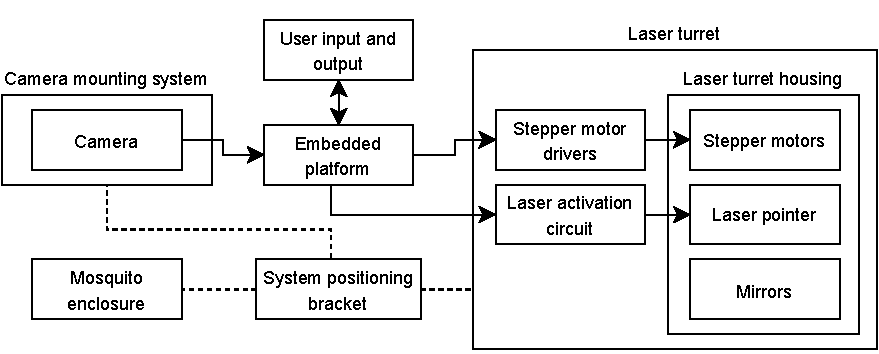
\includegraphics[width=\textwidth]{figures/hardware_block_diagram.pdf}
  \caption{System block diagram.}
\end{figure}

\newpage
\subsection{Record 2.  Systems level description of the design}
The processing for the entire system is done on the Nvidia Jetson Nano. The Jetson Nano reads a frame from the camera. The frame is then processed to detect the position of the mosquitoes and laser reflections. The system updates the mosquitoes tracks. The laser turret target position and the belief position of the laser turret is then updated. The system determines the control action required by the laser turret. The Jetson Nano sends the control signals to the stepper motor drivers. The Jetson Nano is connected to a display, keyboard, and mouse for user interaction. The laser pointer can be powered on and off by the user. The appropriate control signal is sent to the laser activation circuit by the Jetson Nano. The camera, laser pointer, and mosquito enclosure are kept in known positions relative to each other by the system position bracket.

\newpage
\subsection{Record 3. Complete circuit diagrams and description}
\begin{figure}[h]
  \centering
  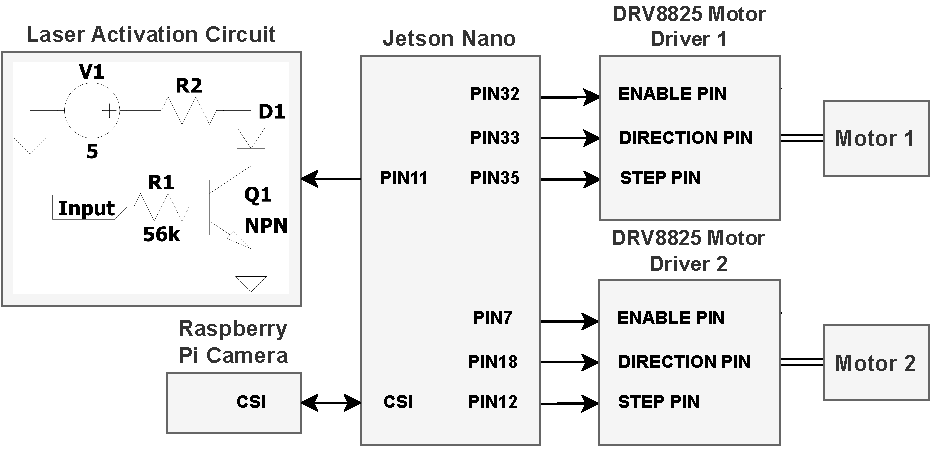
\includegraphics[width=\textwidth]{figures/all_system_connects.pdf}
  \caption{All modules of the system.}
  \label{fig:all_connects}
\end{figure}
\autoref{fig:all_connects} shows a hardware diagram of all the system modules. The laser activation circuit is a switching transistor circuit. The design of the laser activation circuit can be seen in \autoref{par:laser_activation} of \autoref{subsubsec:laser_turret_design}. It was not required to develop circuits for any other modules of the system. The double line connecting the motors and motor drivers represent the connection of the four phases of a bipolar stepper motor.

\newpage
\subsection{Record 4. Hardware acceptance test procedure}
The following procedure should be followed to ensure that system is powered and functioning correctly:
\begin{enumerate}
  \item Confirm that all the hardware modules of the system are correctly connected as shown in \autoref{fig:all_connects}.
  \item The system must be powered using an 8 to 28\,V power supply that can provide at least 15\,W of power.
  \item After the system is powered, the power LED on the Jetson Nano should be on.
  \item The Jetson Nano should be connected to a display, keyboard, and mouse.
  \item Launch the system application as described in \autoref{subsec:software_user_guide}. Manually moving the laser pointer with the \texttt{w,a,s,d,} keys should confirm that the system is functioning correctly.
\end{enumerate}

\newpage
\subsection{Record 5. User guide}
\begin{enumerate}
  \item Confirm that all the hardware modules of the system are correctly connected as shown in \autoref{fig:all_connects}.
  \item The system must be powered using an 8 to 28\,V power supply that can provide at least 15\,W of power.
  \item After the system is powered, the power LED on the Jetson Nano should be on.
  \item The Jetson Nano should be connected to a display, keyboard, and mouse.
  \item The hardware setup is now complete. The system application can be launched as described in \autoref{subsec:software_user_guide}.
\end{enumerate}


%% --------------------------------------------------------------------

\newpage
\section{SOFTWARE part of the project}
\subsection{Record 6. Software process flow diagrams}
The software process flow diagram for the system can be seen in \autoref{fig:tec_software_flow_diagram}.
\newpage
\begin{figure}[H]
  \centering
  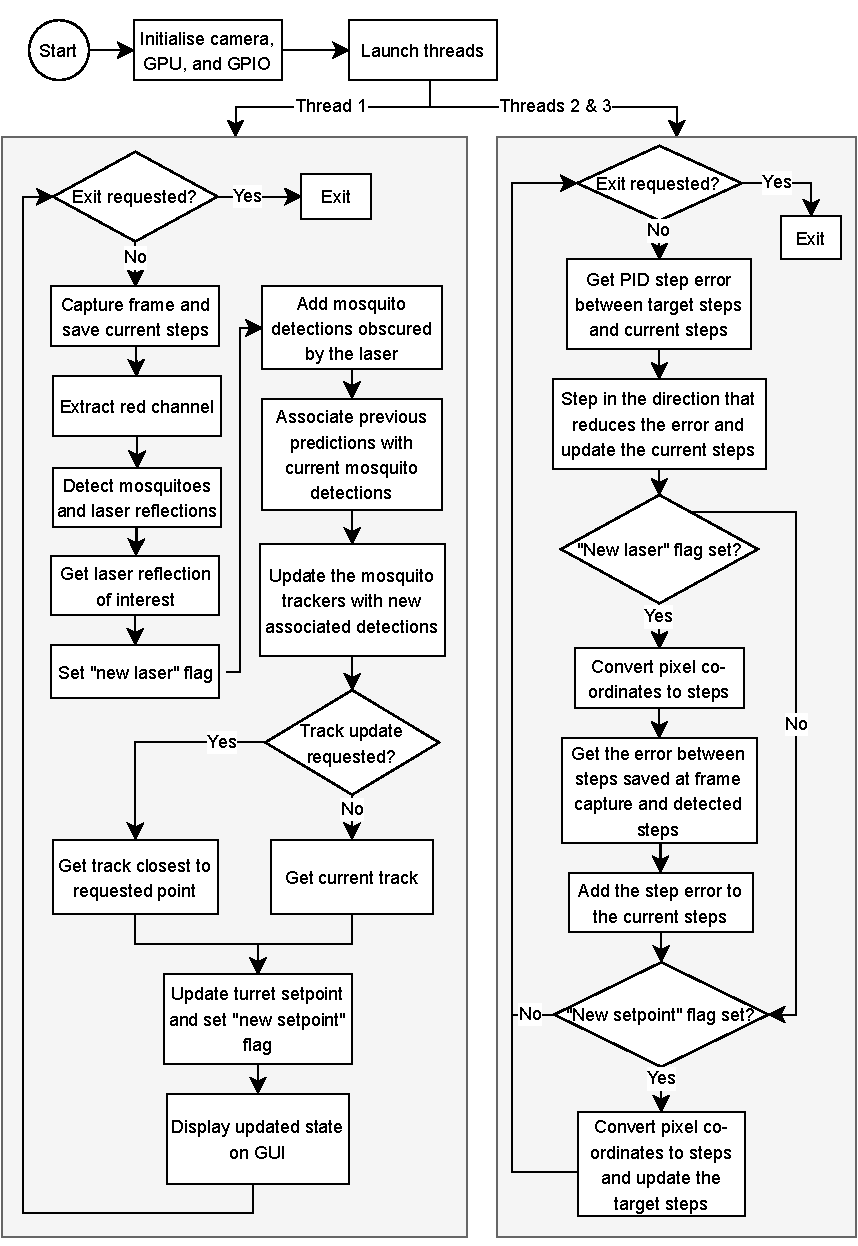
\includegraphics[width=\textwidth, height=\textheight, keepaspectratio]{figures/software_flow_diagram.pdf}
  \caption{Software flow diagram.}
  \label{fig:tec_software_flow_diagram}
\end{figure}

\newpage
\subsection{Record 7. Explanation of software modules}
The software developed for this system is an integrated system. The software flow diagram for the system can be seen in \autoref{fig:tec_software_flow_diagram}. The system starts by initialising the camera, the \gls{gpio}, and the \gls{gpu}. The multiple threads of the system is then launched that are responsible for operating the entire system. Thread 1 is where the main processing of the system occurs and threads 2 and 3 are responsible for controlling the two axes of the laser turret. Communication across the threads is done using atomic variables. All the threads are contained with a loop that continues unless as system exit is requested. This is required to ensure a graceful exit of the system.

Thread 1 is used to interface with the camera. It performs the image processing required for the mosquito and laser detection on the \gls{gpu} and the mosquito tracking. It then updates the detected laser position and target position and sets system flags to indicate this.

Threads 2 and 3 are identical and control the two axes of the laser turret independently. These threads determine the control action required to move the laser turret to the target position. They continuously loop to create the pulses required to move the steppers according to the control action. In this loop the system flags are polled in each iteration. If the system flags indicate that the target position has changed or that the detected laser position is updated, the control action is recalculated. The loop that sends the pulses to the stepper motor drivers is then resumed.

\newpage
\subsection{Record 8. Complete source code}
Complete code has been submitted separately on the AMS.

\newpage
\subsection{Record 9. Software acceptance test procedure}
After the software has been launched, the main system \gls{gui} should appear on the screen. The \gls{gui} should indicate that the laser pointer is powered off, and the system is in \texttt{MANUAL MODE}. After the laser pointer has been powered on and positioned to within the camera frame, the user should change the system to \texttt{FULL AUTO MODE}. The live tracking on the main system \gls{gui} and laser targeting of mosquitoes in the enclosure will indicate that the system is functioning correctly.

\newpage
\subsection{Record 10. Software user guide}\label{subsec:software_user_guide}
\begin{enumerate}
  \item Once the system is launched, use the main system \gls{gui} to confirm that the system is in \texttt{MANUAL MODE}.
  \item Use the terminal interface to manually position the laser, with the \texttt{w,a,s,d,} keys, to within the camera frame. The laser pointer should be powered on at any time during this process as deemed appropriate by the user to ensure the safe operation of the system.
  \item Switch the system to \texttt{FULL AUTO MODE} using the \texttt{k} command in the terminal interface. This will start the automated tracking and targeting of the mosquitoes in the enclosure.
  \item The user can use the mouse to click on any location in the main system \gls{gui}, that will be displaying the live tracking and targeting of the mosquitoes. The system will target the mosquito that is closest to the clicked location.
  \item The user can further interact with the system by using the \texttt{?} command to view all the available control and display commands.
  \item The system can be exited at any point in its operation by using the \texttt{CTRL\,+\,c} command in the terminal interface.
\end{enumerate}

The main system \gls{gui} can be seen in \autoref{fig:tec_main_gui}.


%% End of File.


